% プロジェクト学習中間報告書書式テンプレート ver.1.0 (iso-2022-jp)

% 両面印刷する場合は `openany' を削除する
\documentclass[openany,11pt,papersize]{jsbook}
  
  % 報告書提出用スタイルファイル
  \usepackage[final]{funpro}%最終報告書
  %\usepackage[middle]{funpro}%中間報告書

  % 画像ファイル (EPS, EPDF, PNG) を読み込むために
  \usepackage[dvipdfmx]{graphicx,color}
  
  % ファイル分割のためのパッケージ
  \usepackage{subfiles}
  
  % ここから -->
  \usepackage{calc,ifthen}
  \newcounter{hoge}
  \newcommand{\fake}[1]{\whiledo{\thehoge<70}{#1\stepcounter{hoge}}%
    \setcounter{hoge}{0}}
  % <-- ここまで 削除してもよい
  
  % 年度の指定
  \thisYear{2017}
  
  % プロジェクト名
  \jProjectName{ビーコンIoTで函館のまちをハックする}
  
  % [簡易版のプロジェクト名]{正式なプロジェクト名}
  % 欧文のプロジェクト名が極端に長い(2行を超える)場合は、短い記述を
  % 任意引数として渡す。
  %\eProjectName[Making Delicious curry]{How to make delicious curry of Hakodate}
  \eProjectName{Leverage the Beacon IoT in Hakodate Real Downtown for Our Smarter Life}
  
  
  % <プロジェクト番号>-<グループ名>
  \ProjectNumber{8-A}
  
  % グループ名
  \jGroupName{Hako-B}
  \eGroupName{Hako-B}
  
  % プロジェクトリーダ
  \ProjectLeader{1015253}{橋場保鷹}{Hodaka~Hashiba}
  
  % グループリーダ
  \GroupLeader  {1015053}{佐藤秀輔}{Shusuke~Sato}
  
  % メンバー数
  \SumOfMembers{4}
  % グループメンバ
  \GroupMember  {1}{1015050}{北原康太}{Kota~Kitahara}
  \GroupMember  {2}{1015053}{佐藤秀輔}{Shusuke~Sato}
  \GroupMember  {3}{1015157}{小笠原瑠奈}{Runa~Ogasawara}
  \GroupMember  {4}{1015204}{小島雄士}{Yuji~Kojima}
  
  % 指導教員
  \jadvisor{松原克弥,藤野雄一,鈴木恵二,奥野拓}
  % 複数人数いる場合はカンマ(,)で区切る。カンマの前後に空白は入れない。
  \eadvisor{Katsuya~Matsubara,Yuichi~Fujino,Keiji~Suzuki,Taku~Okuno}
  
  % 論文提出日
  \jdate{2018年1月19日}
  \edate{January~19, 2018}
  
  \begin{document}
  %
  % 表紙
  \maketitle
  
  %前付け
  \frontmatter
  
  % 和文概要
  \begin{jabstract}
  
  % プロジェクト全体の日本語概要
  \subfile{common/common-jabstract}
  
% プロジェクト全体の日本語概要

本グループでは、函館バスの利用がうまくできていないという問題点に目をつけ函館バスを快適に利用することができるアプリケーションの開発を行うこととした。
問題点を下に、私達はどのようにビーコンを用いてバス利用を改善していくかを担当の教員の方からレビューを受けながらアイディアを固めた。
そのアイディアなどを下にサービス設計を行い、後期の活動から開発をするための準備を行った。
7月14日に行われた中間発表会ではビーコンの特性を活かしきれていないのではないかとの指摘もあり、よりビーコンの強みを活かした設計が必要だという課題が見つかった。
後期の活動では前期の中間発表で出てきた問題点をどのように解決するかを話し合うことから始め、開発の方針を固めた。
グループのメンバー全員で10月末までアプリの開発を行いそこからはポスターの作成を行う班とで分かれて作業を行った。
11月10日のデモ発表会では自分たちのアプリをプロジェクトの担当教員にポスター付きで発表を行った。
デモ発表では、ポスター、アプリとともにより修正しなければならない点が多く発見され今後の開発などの目標を固めメンバーでその修正点をどのように修正するのかを話し合い修正、開発を行った。
最終発表では中間発表、デモ発表で言われた点を修正し、発表を行うことができた。

% 和文キーワード
\begin{jkeyword}
ビーコン, フィールドワーク, 函館バス, アプリケーション, 設計
\end{jkeyword}
\bunseki{佐藤秀輔}
\end{jabstract}

%英語の概要
\begin{eabstract}

% プロジェクト全体の英語概要
 \subfile{common/common-eabstract}
 % グループの英語概要

In this group, we decided to focus on the problem that utilization of Hakodate bus was not done well and to develop services.
From that point, we accepted reviews from teachers in charge how to improve the use of the bus by using beacons while consolidating ideas.
We designed the service based on the idea etc. and prepared for development from the latter term activities.

In the interim presentation held on July 14th, there was a case that the characteristics of the beacon could not be fully utilized, and a problem was found that it is necessary to design with the advantage of Beacon more.
In the later activities, we began discussing how to solve the problems that appeared in the interim announcement of the previous term and strengthened our development policy.
All the members of the group worked separately from the team that developed the application until the end of October and created a poster from that.
At the demonstration presentation on November 10, we presented our own app with a poster to the teacher in charge of the project.
In the demonstration announcement, many points to be corrected along with the poster and the application were discovered many times, the goals such as future development were consolidated, the discussion and the development were carried out to discuss how to correct the correction point in the member.
In the final presentation, I was able to correct the points mentioned in the interim announcement, the demo announcement, and make a presentation.

% 英文キーワード
\begin{ekeyword}
Beacon, Fieldwork, Hakodate's Bus, Application, Design
\end{ekeyword}
\bunseki{佐藤秀輔}
\end{eabstract}

  
  \tableofcontents% 目次
  
  
  \mainmatter% 本文のはじまり
  
  % プロジェクト共通の項目
  \subfile{common/common-chapters}
  
  
  
  % グループごとの項目
  
  \chapter{本グループについて}


\section{\midorfin{函館バスの現状と従来のIT利用例}{背景}}

函館市の交通手段として車、市電、バスなどがある。その中でもよく活用する移動手段としてバスがある。バスは気軽に利用でき、車を持っていない人は必然的に利用回数が多くなる。また、バスの時刻表やバスの接近情報を表示する既存のウェブサイトやアプリケーションが存在しているがGPSを用いているため、局所的なバスやバス停の位置の把握に誤差が生じる場合がある。

\bunseki{小島雄士}

\section{函館バスが抱える問題点}

フィールドワークやブレーンストーミングなどの話し合いをした結果、バス停についての問題点、バスの情報を発信しているウェブサイトについての問題点が見つかった。\\
まず、バス停についての問題点は2つ見つかった。
1つ目の問題点は、バスは函館に馴染んでいるが、函館のバス停の中にはわかりにくいものも多いという点である。例えば、「五稜郭」というバス停は同じ名前のバス停が近くに八つ存在している(図3.1)。
これは観光で初めて利用した人にとっても地元住民にとっても分かりにくい。
また、路線が完全に一致しているが往と復で別系統となっている路線も存在し、系統番号だけでは判断できず、バスの乗り間違え、目的のバスがどこに止まるか分からず乗れない、といった問題があげられる。
2つ目の問題点は、似たような名前のバス停が多い点である。前、入口、裏などがあり分かりにくい停留所も存在している。
このためバス停の名前を把握していない人にとって、目的地へ行くためにどこで降りればよいのか分かりにくい、という問題があげられる。\\
次に、バスの情報を発信しているウェブサイトの問題点は2つ見つかった。
まず1つ目の問題点は、バスの接近情報が正確ではない時がある、という点である。
理由は、バスに搭載されている機器がGPS衛星と定期的に通信するため、バスの位置を即位するときに誤差が生じるからである。
さらに大雨の時、渋滞の時、冬に雪が降っている時などは接近情報が「調整中」となり正確な情報を取得できない場合がある。
2つ目の問題点としては、ウェブサイトを利用して目的地を検索することが難しい点である。
あるページはバス停の名前が分からない人のためにマップから検索することができる仕組みとなっている。
しかしマップから選択する時、広範囲な地域選択しかできない。
選択後は目的地候補名が一覧表示されるが、その目的地一覧にない場所へ行きたい時は利用することができない。

\bunseki{小島雄士}

\section{目的}\label{sec:gaiyou}
本グループでは「バス、バス停にビーコンを設置し、函館バスの乗降のミスを少なくする」ことを目的とした。
3.2項であげたように本グループはバス停留所やバスの情報を発信しているウェブサイトについて、いくつかの問題点を発見した。
これらの問題点を解決するために、函館のバスをより使いやすくするアプリケーションの開発を行う。
特に、函館のバスを初めて利用した人にも使いやすいようなアプリケーションを目指す。

\bunseki{小島雄士}

\begin{figure}[htbp]
  \begin{center}
    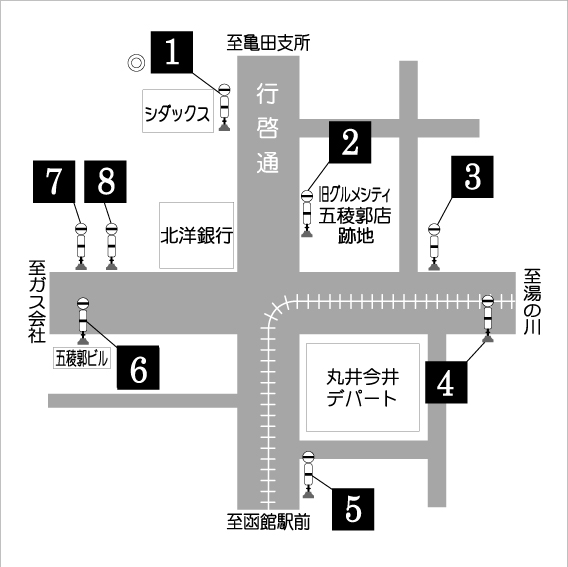
\includegraphics[clip,width=7.0cm]{img/14007.jpg}
    \caption{五稜郭バス停}
    \label{fig:goryo}
  \end{center}
\end{figure}

\chapter{Hako-Bについて}

\section{Hako-bの概要}
Hako-bは、ターゲットを函館バスを初めて使う観光客へ向けたサービスである。
初めて函館に来た観光客でも迷うことなく函館のバスに乗ることができれば、地元の方にも分かりやすいサービスとなるため、観光客にターゲットを当てた。
函館バスの分かりづらい点として、3.2項であげた問題のほか、路線が完全に一致しているが往と復で別系統となっている路線も存在し、系統番号だけでは判断できない。
それらを解決するために私達はHako-bを提案する。
Hako-bのサービスの概要はバス、バス停にビーコンを設置し、バス利用者が乗車予定のバスの系統番号や行き先情報を既存のバスロケーションシステムや時刻表を見なくても乗車できることを目的としたアプリケーションサービスである。
\bunseki{北原康太}


\section{Hako-bの機能}
観光客がHako-bアプリを起動すると、GPSを用いてマップから降車位置を選択でき、降車位置決定後、現在位置の周りにあるバス停を選択することができる。
その後、現在位置から乗車予定のバス停までの経路表示をする。乗車予定のバス停に近づくと、バス停に設置してあるビーコンから「乗車予定のバス停に近づきました。」というPush通知が送られ、近くにバス停が複数ある場所でも、迷わずに乗車するバス停にたどり着くことができる。
そして、バス停に乗車予定のバスが到着した際には「乗車するバスが到着しました。バスに乗ってください。」というPush通知が送られて、複雑な系統番号や降車地が書かれていないバスでも間違うことなく正しいバスに乗れる。

\bunseki{北原康太}

\subsection{機能一覧}
本アプリケーションの機能は、主に5種類の機能がある。以下にそれぞれの機能について述べる。
\begin{enumerate}

\item バス停の選択\\
バス停の名前や位置が紛らわしく分かりにくいものが多い、という問題の解決のために経路を表示した。
位置が分かりにくい、という問題点の例として、五稜郭があげられる。
五稜郭のバス停は五稜郭の周辺に8つ存在しており、どの施設の前にあるか、という違いによって名前が違う。
このようにバス停が多く、しかも交差点を跨いで存在していると位置が分かりにくく初めての人は目的のバスを乗り過ごしてしまう可能性がある。
そこで本アプリには経路表示の機能を入れた。これによってバス停までの道のりが分かるようになった。
経路は現在地からユーザが設定した乗車地までを赤くマップ上に表示する。
また、最短距離を表示するものとした。
\item 経路表示\mbox{}\\
函館バスが抱える1つ目の問題点として、観光や仕事などで始めて函館に来た人が直面する問題点がある。
それはバス停の名前や位置が紛らわしく分かりにくいものが多いということである。
例えば、赤川というバス停がある。
赤川という場所にあるバス停は赤川入口、赤川小学校前、赤川貯水池などのように赤川という名前が入っているバス停が3つ存在している。
函館になれていない人にとっては紛らわしい。
そこで、乗車するバス停を選択する際にマップからバス停を選択できるようにした。
これによって函館へ初めて来た人にも使いやすくなるようにした。
また、マップからバス停を選択することができるのでバス停の名前が複雑な場合も乗車地を選択しやすい。
しかし、バス停を設定する際にいくつもバス停がある場所であると設定することが難しい。そのため複数のバス停がある五稜郭、函館駅前についてはマップ上にピンを1つしか建てない。
しかし内部では設定されており、バス停までの大まかな案内ではなくビーコンを使用した細かな案内もできるようになっている。
観光案内などでバス停の名前は分かるが位置を知らない場合には検索をすることでバス停を絞り込み、場所が分かるようにした。
\item バス停の正誤判定\mbox{}\\
函館バスが抱える2つ目の問題点として、函館では同じまたは似ている名前のバス停が複数存在している、という問題点がある。
例えば、函館駅前のバス停は1番乗り場から7番乗り場まであり、その次は13番乗り場となっている。
これは普段使わない人にとってはどのバス停を使えば良いのか分かりにくい。
さらにこれらのバス停はお互いの距離が近くに存在しているので経路表示では十分な表示ができない可能性がある。
そこで私たちは、バス停に設置されているビーコンの電波範囲内に入った際にアプリがユーザに通知を行うようにした。
近づいたバス停が乗車地に設定したものであった場合は正しいという通知を行う。
同じ、または似ている名前のバス停が近くに存在する場合、乗車地に設定していないバス停に近づくと誤っているという通知を行う。
この通知によって、同じ、または似ている名前のバス停が複数存在していてもユーザは迷うことなく設定したバス停を見つけることができる。
また、このバス停判別機能はビーコンの局所性を最も活用している機能である。
GPSによる測位では誤差が大きく、300m近くの誤差が生まれることもある。
この誤差の範囲内にバス停が複数存在した場合バス停を正確にユーザに通知できない。
しかしビーコンは誤差が大きい場合でも数メートル程度のためバス停を正確に検知することができる。
\item バスの通知\mbox{}\\
函館バスが抱える3つ目の問題点として、目的地に行くためのバスの系統が分かりにくい、という問題点がある。
例えば、はこだて未来大学へ行くバスには105,55,55-1という3つの系統がある。
このように同じ目的地でも複数の系統が存在している。
この問題を解決するために、設定した降車地へ行くバスが接近した際にユーザに通知を行うようにした。
目的のバスが接近し、ビーコンの電波範囲内に入った際に通知を行う。
設定していないバスが接近したときには通知を送らないようにしている。
函館バスは系統が多いが、本アプリからの通知によって、バスの系統を気にすることなくユーザはバスを利用することができる。

\end{enumerate}

\bunseki{小島雄士}

\section{サービス設計}

\subsection{システム概要}
本システムは、バス、バス停に設置されたビーコンにより、そのバス、バス停の正誤判定をするというシステムである。
主な機能としては、目的のバス、バス停に近づいた際にPush通知を送るというものである。
また、Push通知を送るだけでなく、近くのバス停をマップから選択し、時刻表などを確認することができ、利用者が簡単にバスの情報を集めることができる。

\bunseki{佐藤秀輔}

\subsection{ユースケース}
システムとユーザ間でどのような処理が必要になるのか確認するためにユースケースを作成した。
それを元にユースケース図を作成した(図4.1)。
アクターである観光者はアプリを起動し、目的地、現在地付近のバス停を選択する。
選択したのち、ユーザが選択したバス停のビーコンの範囲内に入るとPush通知を受け取る。
その後、目的地まで向かうバスに設置されたビーコンの範囲内に入るとPush通知を受け取る。

\begin{figure}[htbp]
  \begin{center}
    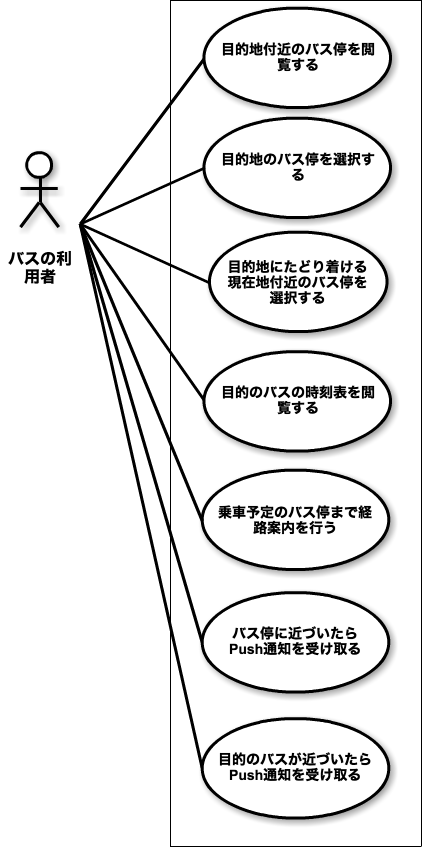
\includegraphics[clip,width=5.0cm]{img/usecase.png}
    \caption{ユースケース図}
    \label{fig:usecase}
  \end{center}
\end{figure}
\bunseki{佐藤秀輔}


\chapter{開発プロセス}
\section{本グループの目標}
本プロジェクトにおける目標は、ビーコンを用いて函館のバス利用をより快適にできるようなアプリを作成することである。
本グループでは「Hako B」のアプリでバス、バス停の判別をでき、乗り間違いを少なくできるような提案、開発をすることを目標とする。

\bunseki{佐藤秀輔}

\subsection{前期活動における目標}
前期の活動での目標は、開発するアプリで、どのように函館バスの利用を快適にできるのかを考え、後期の開発へ向けアプリ機能の洗い出し設計を行うことである。
そのため、函館バスを利用する際にどのような点が不便であるか、またビーコンを用いてどのような問題点を解決できるかを考え、アプリに実装する機能を決める。
後期での開発を円滑に行うため、実装する機能を元にどのような画面遷移をするか、どのようなシステムにするのかを考え、画面遷移図などを作成する。

\bunseki{佐藤秀輔}

\subsection{後期活動における目標}
後期活動での目標は、前期活動にて考案した機能を実装し、実証実験まで行うことである。
前期活動にて考案した機能は以下である。
\begin{itemize}

\item バス停までの経路案内
\item バス停の正誤判定通知
\item 乗車予定バスの通知

\end{itemize}

\bunseki{佐藤秀輔}

\section{開発に用いたツールとその経緯}
\subsection{Xcode}
今回のアプリ開発ではAndroid、iOSの両方の開発をすることが難しいためiOSのアプリ開発を行うこととした。
そのためアプリ開発には、Apple社が開発したXcodeと言うソフトウェアを使用して開発することにした。
開発言語はSwiftを使用した。
使用したバージョンはXcode8.3、Swift3.0の環境で開発をした。
XcodeにはInterfaceBuilderという機能があり実際にコードを書かなくても視覚的にUIを作成する機能があり、リファレンスなど充実しているため開発ツールにXcodeを選択した。
また、Xcode上でシミュレータを起動し実際にiPhoneで動かしているかのようなデバック機能があるため実際にiPhoneを持っていたりしなくても現在のコードを確認できるというメリットも有る。

\bunseki{佐藤秀輔}

\subsection{Git/GitHub}
ソースコードのバージョン管理ツールとしてGit/GitHubを使用した。
Gitは分散型のバージョン管理システムの一つであり、すべてのファイルの変更履歴を含む完全なリポジトリの複製を保存できるというものである。
その為、一度編集したファイルを元に戻すことやどのような編集が行われたのか表示することが可能となる。
リポジトリにはネットワーク上に保存されているリモートリポジトリと、メンバーそれぞれのPC内に保存されているローカルリポジトリの2種類がある。
リモートリポジトリではメンバーそれぞれのファイルの変更履歴を保存し確認、共有することができる。
GitHubとはリモートリポジトリを提供するサービスの一つである。
これにより、複数のメンバー間でスムーズにファイルを共有し開発することが可能となった。

\bunseki{佐藤秀輔}

\subsection{Adobe Illustrator}
ポスターの作成にはAdobe Illustratorを使用した。
IllustratorはAdobe Systemsが販売しているベクター編集ツールで、イラストやポスターなど作成することができるツールである。

\bunseki{佐藤秀輔}

\section{環境構築}
Xcodeを使用するためにまずはAppleIDの作成が必要だったため個人が持っているアカウントもしくは開発のためにAppleアカウントを作成を行った。
開発の環境としてはXcodeのインストールを行うことで整うためXcodeのインストールを行った。
GitHubに関しては、リモートリポジトリに機能の追加、バグの修正などの種類ごとにブランチを作成し、そこへプッシュするようにした。
developなどの開発用のブランチを作成せずにmasterにマージする際にテストを行い問題がないかレビューを行いmasterにマージをするという手法で行った。
masterにマージする際にレビューを徹底することでmasterのファイルでバグが起きないようにすることができる。

\bunseki{佐藤秀輔}

\section{夏休みの活動}
メンバー全員でiOSのアプリ開発の経験がある人が1人しかいなかった為、夏休み中にアプリ開発の基礎的な知識を学習できるような資料の作成を行った。
メンバーには作成した資料に基づき、経験のあるメンバーに質問をしながら基礎的な知識をつけられるように活動を行った。
その際のプログラムの教材として
\begin{itemize}

\item Swiftの基礎知識
\item Hello Worldのプログラム作成
\item TableViewを用いたアプリの作成

\end{itemize}
の3つを題材として基礎的な知識について学習を行った。

\bunseki{佐藤秀輔}

\section{中間発表}
\subsection{発表形式}
始めにメインポスターの発表を5分間行った後、聞き手には3つのサブポスターのどれかを選んでもらいそれぞれ発表を聞いてもらった。
Hako-Bのポスターセッションでは前半と後半それぞれ2人ずつに分かれて発表を行った。
一人は概要、システム構成、今後の予定を話し、もう一人はHako-Bについてを話した。

\bunseki{小笠原瑠奈}

\subsection{発表内容}
始めに、概要を説明した。
まず、Hako-Bを提案するに至った問題点を実際のバス停の例と画像を用いて提示した。
1つ目は同じバス停名が近くに複数存在すること、2つ目は似たような名前のバス停が存在すること、3つ目は目的地に行くためのバスの系統がわかりづらいことだった。
その後、先に述べた問題から生じるミスを解消することを目的とした。次にHako-Bの機能説明をした。
まず、アプリの特徴を箇条書きで大まかに示した。
特徴は3つあり、1つ目は利用者が設定したバス停までの道案内を GPS を用いて行うこと、2つ目はバス停に設置されたビーコンから受けた電波によってバス停への接近を利用者に通知すること、3つ目はバスの車内に設置されたビーコンから受けた電波によってバスの到着を通知することである。
その後、処理フローでイラストやスマホ画面などの画像を用いてアプリの機能を具体的に説明した。
次に、システム構成の説明を行った。
最後に、今後の予定を3つ示した。
1つ目は設計を基にプロトタイプを作成すること、2つ目は模擬バス,模擬バス停による実証実験を行うこと、3つ目はテストで出た問題の改善を行うことである。
以上がポスター発表の内容となる。

\bunseki{小笠原瑠奈}

\subsection{レビュー内容}

\begin{description}
\item[発表方法についての評価と反省]\mbox{}\\
発表技術に関して、プラスの意見として
\begin{itemize}

\item 身振り手振りがあって良い
\item 発表が分かりやすかった

\end{itemize}
などが挙げられ、聞き手に内容を上手く伝えることができたと分かる。以上から発表技術に問題はなかったと言える。
マイナスの意見としては
\begin{itemize}

\item 声が聞き取りづらい
\item ポスターのレイアウトが意味不明
\item 画面遷移図が小さい
\item 図に少し説明を入れると良い

\end{itemize}
などが挙げられた。平均評価は7であった。
以上から、発表する際の各グループの配置や向きを見直す必要があること、ポスターのレイアウトを読み進めやすいものにすること、アプリ画面のテキストをポスター用に大きくすること、図を見やすくして説明を付けることが改善点として挙げられる。

\bunseki{小笠原瑠奈}

\item[発表内容についての評価と反省]\mbox{}\\
発表内容に関しては、プラスの意見として
\begin{itemize}

\item 問題の着目点が良い
\item アプリのニーズは高い
\item 実際に欲しい

\end{itemize}
などが挙げられ、提案に対する聞き手のニーズが高いことがうかがえた。マイナスの意見としては、
\begin{itemize}

\item プロトタイプもできていないので課題が山積み
\item 内容の検討がたりない
\item ビーコンの利点をうまく使いこなせていない。もっと他にも良い活用法があるかもしれない
\item バス停名が分からない人にはどうするのか
\item 計画を具体的に詰めたら良い

\end{itemize}
などが挙げられ、提案システムの問題点や今後の予定が詳細に決められていないことに指摘を受けた。
平均評価は7であった。
以上から、今後出来るだけ早い段階からプロトタイプを作る必要があること、様々なアクターを想定したユースケースを再検討すること、今後の計画を詳細に決めることが改善点として挙げられる。
また、「バス停名が分からない人にはどうするのか」という指摘に対しては、ユーザーが目的地を入力するとマップ上から推奨される降車地と乗車地を選択できるというアプリの機能が解決策となる。
しかし、これは展望であり、実装予定の機能としてはポスターに載せていなかったので説明不足であったと反省する。

\bunseki{小笠原瑠奈}

\end{description}

\section{オープンキャンパス}
はこだて未来大学のオープンキャンパスで本プロジェクトの説明を行った。
説明方法はオープンキャンパスに来た方がポスターの前に立ち止まり見ているときにHako Bについての説明を行う、という方法をとった。
また、Hako Bのポスターははこだて未来大学の学生や先生を対象としたポスターとなっている。
そのためオープンキャンパスに来た人には難しい用語がある。
そのためポスター説明で専門用語を話す際にはその都度用語の説明をした。

\bunseki{小島雄士}

\section{デモ発表会}
\subsection{内容}
発表会ではポスター、実機を用いて説明を行った。最初にポスターの説明を行った。
デモ発表会のため、ポスターの説明は簡略化して行い、デモの説明を多くした。
まずHako Bの概要を説明した。
その後、実機の画面をプロジェクターで投影してデモを見せながらアプリの機能を説明した。
前期のポスターとの違いとして、既存のアプリとの差別化をした点を新しく入れた。
デモ発表会の時点ではまだ、経路表示、乗車地に設定していないバス停についた時の誤り判定はなかった。

\subsection{レビュー}
デモ発表会のレビューは「デモの完成度は高かったですか」「ポスターはわかりやすかったですか」の2項目に分けてレビューを行った。
それぞれ、「わかりにくかった」から「わかりやすかった」まで5段階で評価を受けた。
また、それぞれ改善点やコメントをした。\\
 デモに対しての評価としては5段階評価で平均3.3となった。また、コメントには以下のようなものがあった。
\begin{itemize}

\item この時期にしてはかなり進んでいる状態だと思います。ただ、もっと欲を言うとUIにこだわれるようになるといいと思います。
\item 機能も見た目も割と出来ているように見えました。
\item 亀田支所や五稜郭前など分かりやすい場所のデモをするとわかりやすい。
\item 複数個バス停があるので乗りやすいというのがアピールポイントだと思うので、早めに経路表示を実装した方がいいと思います。
\item もう少しストーリー性があると良いと思った。

\end{itemize}

以上のコメントより、アプリの機能面に関しては実装が進んでいる。
また、アプリの見た目に関しても分かりやすいものになっていると思われる。
デモの改善点としてはより分かりやすいデモを行うことが必要だと言える。
コメントにあるように、亀田支所や五稜郭を使用してデモを行うと分かりやすいと感じた。
また、経路表示の実装を早めにすると説明も分かりやすくなる。
また、初めてHako Bを初めて見た人に対して、アプリの有用性を説明することも大切だと思われる。
今回は同じプロジェクト内でのレビューなのである程度概要を知っている状態でレビューをした。
しかし、初めて見る人に対してはビーコンをどこに使っているのか、どのような流れでアプリを使えばいいのか、といったHako Bの説明がまだまだ足りていないと思われる。\\
 ポスターに対しての評価としては5段階評価で平均3.3となった。また、コメントには以下のようなものがあった。
\begin{itemize}

\item 全体的に見やすかった。
\item 機能ごとに画面を表示しているのが良い。既存のアプリとの違いの欄に不自然な空白があるのが気になった。
\item 人が物事を理解するときは、Whyの説明がかなり重要です。機能が必要な理由を述べられると良いです。
\item 目的や背景がないので動機が分かりづらい。
\item 全体的に図と説明が足りない。ポスターからはHako Bの魅力が伝わらないので、Hako Bとはの部分をもう少し説明を濃くした方がいいかもしれないです。もしくは、全体の流れを表す図を入れた方がいいと思います。
\item テキストが多いと感じた

\end{itemize}
以上のコメントより、作成したポスターはシンプルだったと考えられる。
デモの改善点としては主に見た目に関してのものが多かった。
例えば図が少ない、不自然な空白がある、テキストが多いなどがあげられる。
また、目的や背景を入れていなかったため、動機が分かりづらい、というコメントもあった。
Hako Bの機能が必要な理由が足りていない、Hako Bについての説明が少ない、などのコメントより、デモと同じようにアプリについての説明が不十分だったと考えられる。
アプリの図もただ4つあるだけだと順番に並んでいても気が付かないので矢印や数字などを使って見やすくするように改善したい。

\bunseki{小島雄士}

\section{金沢工業大学の教授に対しての発表}
来ていただいた教授の方々に向けてポスターを使用して発表した。時間が限られていたため3分程度で説明をした。
まず、Hako Bの概要を説明した。
その後簡略化してアプリの使用フローやアプリ画面を説明した。
最後に今後の展望を発表した。
発表では時間が限られていたためゆっくりと時間を取って詳しく話すことができなかったが要点は十分に発表することができた。

\bunseki{小島雄士}

\section{最終成果発表}
\subsection{発表形式}
始めにプロジェクト全体の発表をスライドで 5 分間行った後、聞き手に 3 つのサブポスターのどれかを選んでもらい発表を聞いてもらった。
Hako-B のポスターセッションは中間発表と同じ形式で、発表者の組み合わせも同じであったが、同時にアプリのデモを行った。
一人は問題、Hako Bについて、アプリの使用フロー、学び、展望を話し、もう一人はアプリの機能について実際にアプリを動かして説明した。
デモではアプリがバス停・バスのビーコンを検知することに重点を置き、アプリを動かす方がバス停のビーコンを持ち、もう一人がバスのビーコンを動かすことでプッシュ通知が来る様子を見せた。

\bunseki{小笠原瑠奈}

\subsection{発表内容}
まず概要において、アプリを開発するに至った背景として、「初めて函館に来た人はバス停名・位置が分かりづらい」、「函館では同じまたは似たような名前のバス停が複数ある」、「目的地に行くためのバスの系統が分かりづらい」、以上の3点を函館バスの問題点であると、例えを交えながら提示した。
その後、提示した問題を解決するために開発したという流れでHako Bとはどのようなアプリなのかを簡潔に説明した。
次にアプリの使用フローを軽く説明した後、分かりやすいよう実際にアプリのデモプレイで、マップから乗車地・降車地を選択した後、次の画面で時刻表をタップすると乗車地までの経路が表示されるという流れを軽く示した。
乗車地・降車地選択の画面では検索フォームに「赤川」と入力すると「赤川」が含まれるバス停だけが表示される様子も見せた。
そして「はこだて未来大学」を想定したビーコンをスマホに近づけると「バス停が近くにあります」、違うビーコンを近づけると「違うよ!」と通知され、バスを想定したビーコンが近づくと「バスが到着しました」と通知される様子を見せた。
最後に、後期の活動を経ての学びとして、「Swift での iOS アプリ開発の流れを学んだ」、「Beacon を用いた局所的な位置情報の利用法を学んだ」の2点と、今後の展望として、「正確なバス遅延時間の表示」、「乗り換えも考えたルートの表示」の2点を提示した。

\bunseki{小笠原瑠奈}

\subsection{レビュー内容}

\begin{description}
\item[発表方法についての評価と反省]\mbox{}\\
発表方法に関して、プレゼンに関するプラスの意見として
\begin{itemize}

\item 具体的なシチュエーションでの説明がわかりやすかった。
\item とても効果的なプレゼンが出来ていました。
\item 詳細をしっかり説明してくれている。
\item 詳細をしっかり説明してくれている。
\item 発表する速さが程度良い感じです。

\end{itemize}

などがあった。また、ポスターに関しては
\begin{itemize}

\item ポスターの図が分かりやすかった
\item と内容をまとめられていたため分かりやすかった。

\end{itemize}

などがあり、デモに関しては
\begin{itemize}

\item 発表技術について、体験ができて、理解しやすかった。
\item デモを行っていてわかりやすい。大きめのディスプレイを使っていてわかりやすかった。

\end{itemize}

などの意見をいただいた。次にマイナスの意見に関しては、
\begin{itemize}

\item 少し声が聞き取りにくかった。
\item 声が小さく聞き取りづらかった。
\item パネルセッションなのでパネルかくさない方がよいのでは?

\end{itemize}
など声の通りに対する意見を多くいただいた。
以上から、内容を説明する流れやポスター、デモは高評価であったことから分かりやすく、効果的であったと思われるが声量や動きに問題があったと言える。
平均評価は7.5で、中間発表よりも0.5ポイント上がった。

\bunseki{小笠原瑠奈}

\item[発表内容についての評価と反省]\mbox\\
発表内容について、開発したアプリに関するプラスの意見として
\begin{itemize}

\item はこだてのバスの問題をビーコンで解決しようとした点は、ユニークで面白いと思いました。
\item アプリのデザイン、とても良かった。これまでにない地域に合う案内方法ができると思いました
\item 市民の抱える問題に対する課題解決がテーマになっていて、わかりやすかった。
\item Hako B使ってみたいです。バスは乗らないのですが、このアプリがあれば乗ってみようと思います。
\item Beaconとてもおもしろそうでした。実用化されたら欲しい。
\item アイデアは非常に面白く、欲しいと感じました。
\item このアプリが実装されたらもっと快適に乗ることができると思った

\end{itemize}
などの意見を頂いた。アプリ以外の事柄に関しては
\begin{itemize}

\item 次の課題も把握しているところが良いと思った。
\item 利用の流れがわかりやすかった。
\item メンバーの学びがあるのがよい。

\end{itemize}
などの意見をいただいた。次にアプリに関するマイナスの意見としては、
\begin{itemize}

\item その場所(土地)を全く知らない人にも、やさしいUIとサービスがあるとよいと思いました。(StartとEndがわかっている段階での話に感じました。)
\item 実証実験などをもう少しやると、よいと思いました。
\item 実際に実験をしてシステムとしてなりたつのかを是非確認してほしい!
\item アプリで自分の行きたい目的地を指定してもよりのバス停を指定できるようにしたら良いと思います。(乗車地、降車地を指定してくれる)
\item 質問にあったように時間のずれが分かるといい

\end{itemize}
などの意見を頂いき、アプリ以外の事柄に関しては
\begin{itemize}

\item ビーコンとアプリの関係性(どうやってリンク?させるか等)の説明がなかったので、もう少し動作の中身が知りたい。
\item 学びの部分が苦労したことやどう解決したかなどが知りたかった。

\end{itemize}
などの意見をいただいた。
以上からアプリの有用性は高く、使いたいという意見も多かったことからHako Bに対する評価は高いことが伺えた。
しかし、バス停の選択や時刻表などユーザー任せ、実現できなかった機能に対する指摘も多かったので今後の課題としたい。
アプリ以外では学び、展望に触れていることが好感触だったが、もう少し詳しく説明してほしい、アプリのビーコンの連携など技術的なことに関する説明についても深く触れてほしいという意見もあったので、詳細に説明すべきであったと感じた。
平均評価は8.5で中間発表よりも1.5ポイント上がっていた。

\bunseki{小笠原瑠奈}
\end{description}

\chapter{今後の予定・展望}
\section{今後の予定}
\subsection{プロトタイプの作成}
Hako-bのプロトタイプでは、乗車地までの経路表示、ビーコンを用いた乗車地のバス停に近づいたことを知らせるPush通知機能の実装、乗車するバスがバス停に近づいたことを知らせるPush通知機能の実装をする予定である。
また、既存のバスロケーションサイトとの差別化を考え、中間発表で指摘されたバスの時刻表情報もバスの接近に付随して実装していく予定である。

\bunseki{北原康太}

\subsection{実証実験}
プロトタイプを作成した後にビーコンを設置した模擬的なバス、バス停を見立てシステムが正常に動作するかテストを行う。
その際のテストでは、
\begin{itemize}

\item 実際にどの程度の距離よりビーコンの電波を検知してPush通知が送られてくるのか
\item 車内からのビーコンの電波でどの程度の距離から判別できるのか
\item バスが連なってきた場合のバスの判別
\item バス停が多くある箇所で目的のバス停が判別できるのか

\end{itemize}
これらのビーコンが用いられている箇所の動作を安定させるようなテストを行なっていく予定である。

\bunseki{佐藤秀輔}

\section{後期へ向けての展望}
プロトタイプ作成後、実際のバスとバス停にビーコンを設置するに向けて、フィールドテストをしていきたいと考えている。
具体的な実験方法はバス車内に設置されたビーコンに見立てて実際のバスにビーコンを持って乗車し、バス停に立っているHako-bアプリ利用者にバス接近情報が通知されるかどうか、またバス停付近にビーコンを持って立ち、どの範囲なら乗車予定のバス停がビーコンによって見つけられるかということを検証していきたい。
また、バス停の選択の際にバス停名と位置を知っていなければ選択できないという問題がある。その問題の解決のために、バス停の名前を知らなくても選択できる方法、例えば目的の観光地の名前からバス停を推測するような機能を追加していきたい。

\bunseki{北原康太}

\section{今後の展望}
今後の展望として、GPSを用いたバス遅延時間の計算よりもビーコンを用いて遅延時間の計算をし、より正確な遅延時間の機能の追加をしたい。
具体的な方法として、1つ前のバス停のビーコンの電波を受け取ったユーザの時間とバスの時刻表の時間のズレをサーバで管理し、リアルタイムで遅延表示を行う。
また、バスの乗り換えの実装もしたい。
そして、最終成果発表でいただいた意見より、目的の降車地に着いたバスの通知機能もあると、初めて函館のバスを利用するユーザにとって有益であると分かったため、降車地のPush通知機能も実装したい。

\bunseki{北原康太}


\chapter{まとめ}
\section{前期の振り返り}
前期の活動では、大きく分けてロゴ制作、ビーコンについての学習、フィールドワーク、アイデア出しの4つについて行った。まずロゴの制作ではメンバー各自が考えてきたデザインを持ち寄って、どのような考えでロゴを作成したのかを発表し、投票形式でプロジェクトのロゴを決めた。\\
ビーコンについての学習では、ビーコンの仕組み、種類、またビーコンの活用事例などを調べ、3分間の発表をして、情報を共有した。\\
次に、フィールドワークのための班を決め、フィールドワーク講習会などを受講した。調査内容を決めるなどの事前準備を行い、フィールドワークへ赴いた。行き先は、四稜郭・五稜郭・西部地区の3つのエリアで、観光客や地元民の行動観察、聞き取り調査、現地の資料の収集などを行い、それらの結果をまとめてプロジェクト全体と結果を共有した。\\
その後のアイデア出しでは、アイデアソンを行い、自分が考えて良いと思ったアイデアを1つのスライドにまとめて発表を行った。メンバー各自が出したアイデアを基に3グループに分かれ、アイデアを3つずつ出し、Tangerine株式会社やトランスコスモス株式会社に対して発表を行いレビューをいただいた。

\bunseki{北原康太}

\section{後期の振り返り}
後期の活動では、中間発表でいただいた意見を元に不十分だった点を洗い出し、サービスの見直しをした。
特に、「誰を対象にしたアプリなのか」が明確になっていなかったため、函館のバスを初めて利用する観光客を対象とし、アプリの開発へと進んだ。
11月に行われたアプリのデモ発表会では、レビューをしていただいた先生方から、「なぜビーコンを用いると良いのか」ということを強調するべきだという意見をいただいたので、グループメンバーと話し合い最終成果発表に向けて、ポスター作成と発表練習を行った。

\bunseki{北原康太}

\section{前期の活動での学び}
\subsection{ビーコンについて}
メンバーの大半がビーコンについてほとんど何も知らなかったため、ビーコン勉強会を開いて、現在のビーコンの活用事例やビーコンでできることとできないことについての情報を共有した。
また、ビーコンを取り扱っているTangerine株式会社とトランスコスモス株式会社からプロジェクトメンバーが考えたアイデアについてのレビューをいただき、よりビーコンについての知識を深めた。

\bunseki{北原康太}

\subsection{情報共有・プレゼンテーション技術}
前期の活動で行ったアイデア出しの中でアイデアソンやブレーンストーミング、KJ法を用いて情報や発想をメンバーに共有する方法を学んだ。
短い時間の中でたくさんのアイデアを出すアイデアソンでは、アイデアを星の数で評価し、競い合い、そのアイデアをブラッシュアップさせることによってメンバー同士が納得のいくアイデアが生まれやすかった。
また、Tangerine株式会社とトランスコスモス株式会社に向けて、それぞれのグループで考えたアイデアをプレゼンテーションをした際に、起承転結の構成を強く意識した発表資料を作り、分かりやすいプレゼンテーションになるように心がけた。

\bunseki{北原康太}

\section{後期の活動での学び}
\subsection{チーム開発}
グループメンバーのほとんどがチーム開発をするのが初めてだったため、グループリーダーを中心に適宜、ソースコードのバグや他人が見てもわかりやすい変数名をつけるなど意識して開発を行った。
また、ソースコードを一括管理するツールとして「SourceTree」を利用してGithubのリポジトリの操作を円滑化して作業効率を高めることができた。

\bunseki{北原康太}

\subsection{iOSプログラミング}
グループリーダーを除いてiosプログラミングの経験がなかったため、各自、夏休みなどを利用し、簡単なiPhoneアプリを作成して、学習を進めた。
開発環境である「Xcode」にはiPhoneアプリ画面の遷移や見た目の操作など、UIを考慮しなければならないことも多々あったため、コードの量や画面数が増えるにつれて、理解しづらくならないように、逐一コメントを残すことを心がけた。

\bunseki{北原康太}

\section{個人の振り返り}
\subsection{北原康太}
新規プロジェクトということで実際に函館の街に赴き、観光客の方や地元の方などに聞き取り調査を行い函館の街の不満点や問題点を見つけるというところから、このプロジェクトはスタートした。
問題点からその解決策を見出す難しさを身にしみて感じた。特に、前期に行った「アイデアソン」や「アイデアコンテスト」で短い時間でいくつものアイデアを紙に書き出し、創出した経験は、今後の学生生活や実際の業務に携わった時にも役に立つ手段だと思う。
そして、チーム開発においては、今まで扱ったことのない「Swift」を使用して、バス停関係の開発を担当できた。
チーム開発は、お互いにコミュニケーションをとって相手の開発担当部分を理解するという学習が大いに自分のためになった。
人のソースコードを読んで理解しやすい点・しにくい点を参考にして自分のコードを見直すきっかけになれたこと、ユーザの求める機能がなんであるかをメンバーと考えて開発に携われたことがチーム開発から得られた経験である。

\bunseki{北原康太}

\subsection{佐藤秀輔}
今回のプロジェクトでは函館という一つの地域に目を当ててどこに問題があり、その問題をどのようにビーコンを用いて解決をするのかということを考えるというところが初めての経験だった。
私は、このグループAのグループリーダーとして活動していたが、メンバーをまとめ、メンバーごとに指示を出したりするということがかなり難しいと感じた。
活動の中でグループのメンバーへの指示が遅くなったり、あまり指示を詳しく出すことができていなくメンバーの作業が止まってしまうことがあり、その部分を改善しなければいけないと感じた。
開発に関しては、今回のiOSアプリの開発で自分しか開発の経験がなかったためメンバーがアプリ開発の基礎知識をつけられるように、Swiftの資料などを作成するということをした。
今回のプロジェクト学習を通して、リーダーとしてどのようにメンバーに指示を出していくのか、iOSアプリでのビーコンの扱いの仕方などを学ぶことができ良い経験を得ることができた。

\bunseki{佐藤秀輔}

\subsection{小笠原瑠奈}
サービスを提案して、反応をいただける面白さが印象に残った。
特に、提案するアプリやポスター・発表方法について、中間発表では指摘を受けたのに対し、最終発表では指摘もあったが「アプリを使いたい」「分かりやすい説明」などの肯定的な反応を多くいただけたのが嬉しかった。
また、サービスの提案から設計、開発までシステム開発の一連の流れを体験することができたのは実りになった。
具体的に言うと、フィールドワークやアイデアソンなど課題発掘やアイデア提案の手法を学ぶことができた。
加えて、チーム内での話し合い、コミュニケーション、作業の分担、連携など複数人で取り組む難しさを経験できた。
技術面に関してはあまり上達できなかったがSwiftを少しと、イラストレーターを扱うことができるようになった。
それらを通して得た反省も多く、例えば、課題発掘における関心や経験の無さや、多角的に見ることが上手くなかったためにアイデアの問題点を多く発見することができない、コミュニケーションが足りないので連携が取れない、などが挙げられる。
以上から、プロジェクト学習を通してサービスを提案する楽しさと難しさ、チームで開発することによる多くの反省を得た。
今後はこれらの反省点を経験として、改善することで活かしていきたい。

\bunseki{小笠原瑠奈}

\subsection{小島雄士}
個人の振り返りとしてはSwiftを使用したアプリ開発、Gitの使い方、ビーコンという新しい技術について学ぶことができた点が大きい。
まず、Swiftを使用したアプリ開発を行うことができたのは良い経験となった。
Swiftという今までに使用したことのない言語を学ぶ機会が得られた。
今まではアプリの開発というものをやったことがなく、漠然としたイメージしかなかった。
また、今までに制作したものは全て機能が一つのものだけだったため、本プロジェクトによってアプリ開発を経験できたのはいい機会であった。
次に、Gitを使用できたことも今後の糧となる。
プロジェクト開始以前はGitを使用したことがなく、知識もなかった。
しかしプロジェクト内の講習会や開発によってGitについての理解を深めることができた。
Gitを使用した開発においては、コンフリクトや役割分担などで苦労した。
今までは一人でソースコードを書く機会しかなかったため、チーム開発でのみ起こりうるこれらの苦労を経験することは良い経験となった。
チームでの開発は行ったことがなくチーム開発の大変さや苦労を経験できた。
細かく連絡や進捗の報告をすることがとても大変であり大切なことだと気づくことができた。
将来チームで開発を行う機会はあると思うので、今回の経験を生かしたい。
また、ビーコンという技術に触れることができ、自分の知らなかった知識を得ることができた。
プロジェクト開始以前はビーコンについての知識がほぼなかったがビーコンについて調べ、プロジェクト内での話し合いなどを通して知識を得ることができた。
ビーコンがどのような情報を持った端末なのか、なにをすることができるのかなどを知ることができた。
今後ビーコンなどの位置情報を利用した開発を行う際に今回得た知識を生かしたいと思う。

反省として、ビーコンの端末についての知識を得ることができたが開発に関しては知識が足りなかった。
Swiiftを使用してビーコンから情報を得る方法については完全に理解をすることができず、コードを書くことができなかった。
今後はビーコンを使用する際にビーコンの情報を得る方法を調べ、コードを書くことが出来るようにしていきたい。
通知をアプリからスマートフォンの画面に出す方法は難しく、メンバーの1人に任せてしまった。
また、Xcodeを使用してアプリ開発を行ったが、Xcodeの機能の内一部しか使いこなすことができなかった。
ViewやSearchBar、Label、といった機能を主に使用した。
他の種類のViewやBarがあったのでより良いものがあったかもしれない。
このようにプログラミングや実装の点に関しての反省点は多い。
Gitに関しての反省点もある。
Gitを使用してソースコードのバージョン管理を行ったが、Gitに関しての知識が足りずメンバーに不明な点を質問する機会が何回もあった。
もっと自分での勉強時間を設けることが大切だったと感じた。
ソースコードのバージョン管理の際に誤ってクローンやプッシュをしてしまうとほかのメンバーに迷惑をかけてしまうので注意することが大切だと学んだ。
1度プルをする際に誤ってしまい、メンバーに助けて貰ったことがあった。
この時にはメンバーに助けて貰うまで自分ではコーディングをすることができなかった。
これは時間を余計に使ってしまったと反省する。
怖がってプロジェクトの時間まで何もしないのではなく自分で調べて努力することが必要だった。
プロジェクトが始まって初めて使用する言語や開発環境だったので戸惑うことが多かった。
しかし、Gitは今後使う機会が多いと思われるのでいい経験となった。
これからは自分で学びGitを使う際に戸惑う機会を少しづつ減らしていこうと思う。
次に、当初予定していた機能が完成しなかった点も反省したい。
当初はデータベースを使用し多くのバス停の情報を使用する予定だったがデータベースの導入が間に合わなかったため使用することができなかった。
今後はデータベースについても調べ、機会があれば使用することが出来るようにしたい。

\bunseki{小島雄士}


  % 以降、付録(付属資料)であることを示す
  \begin{appendix}
  
\chapter{画面遷移図}
\begin{figure}[htbp]
  \begin{center}
    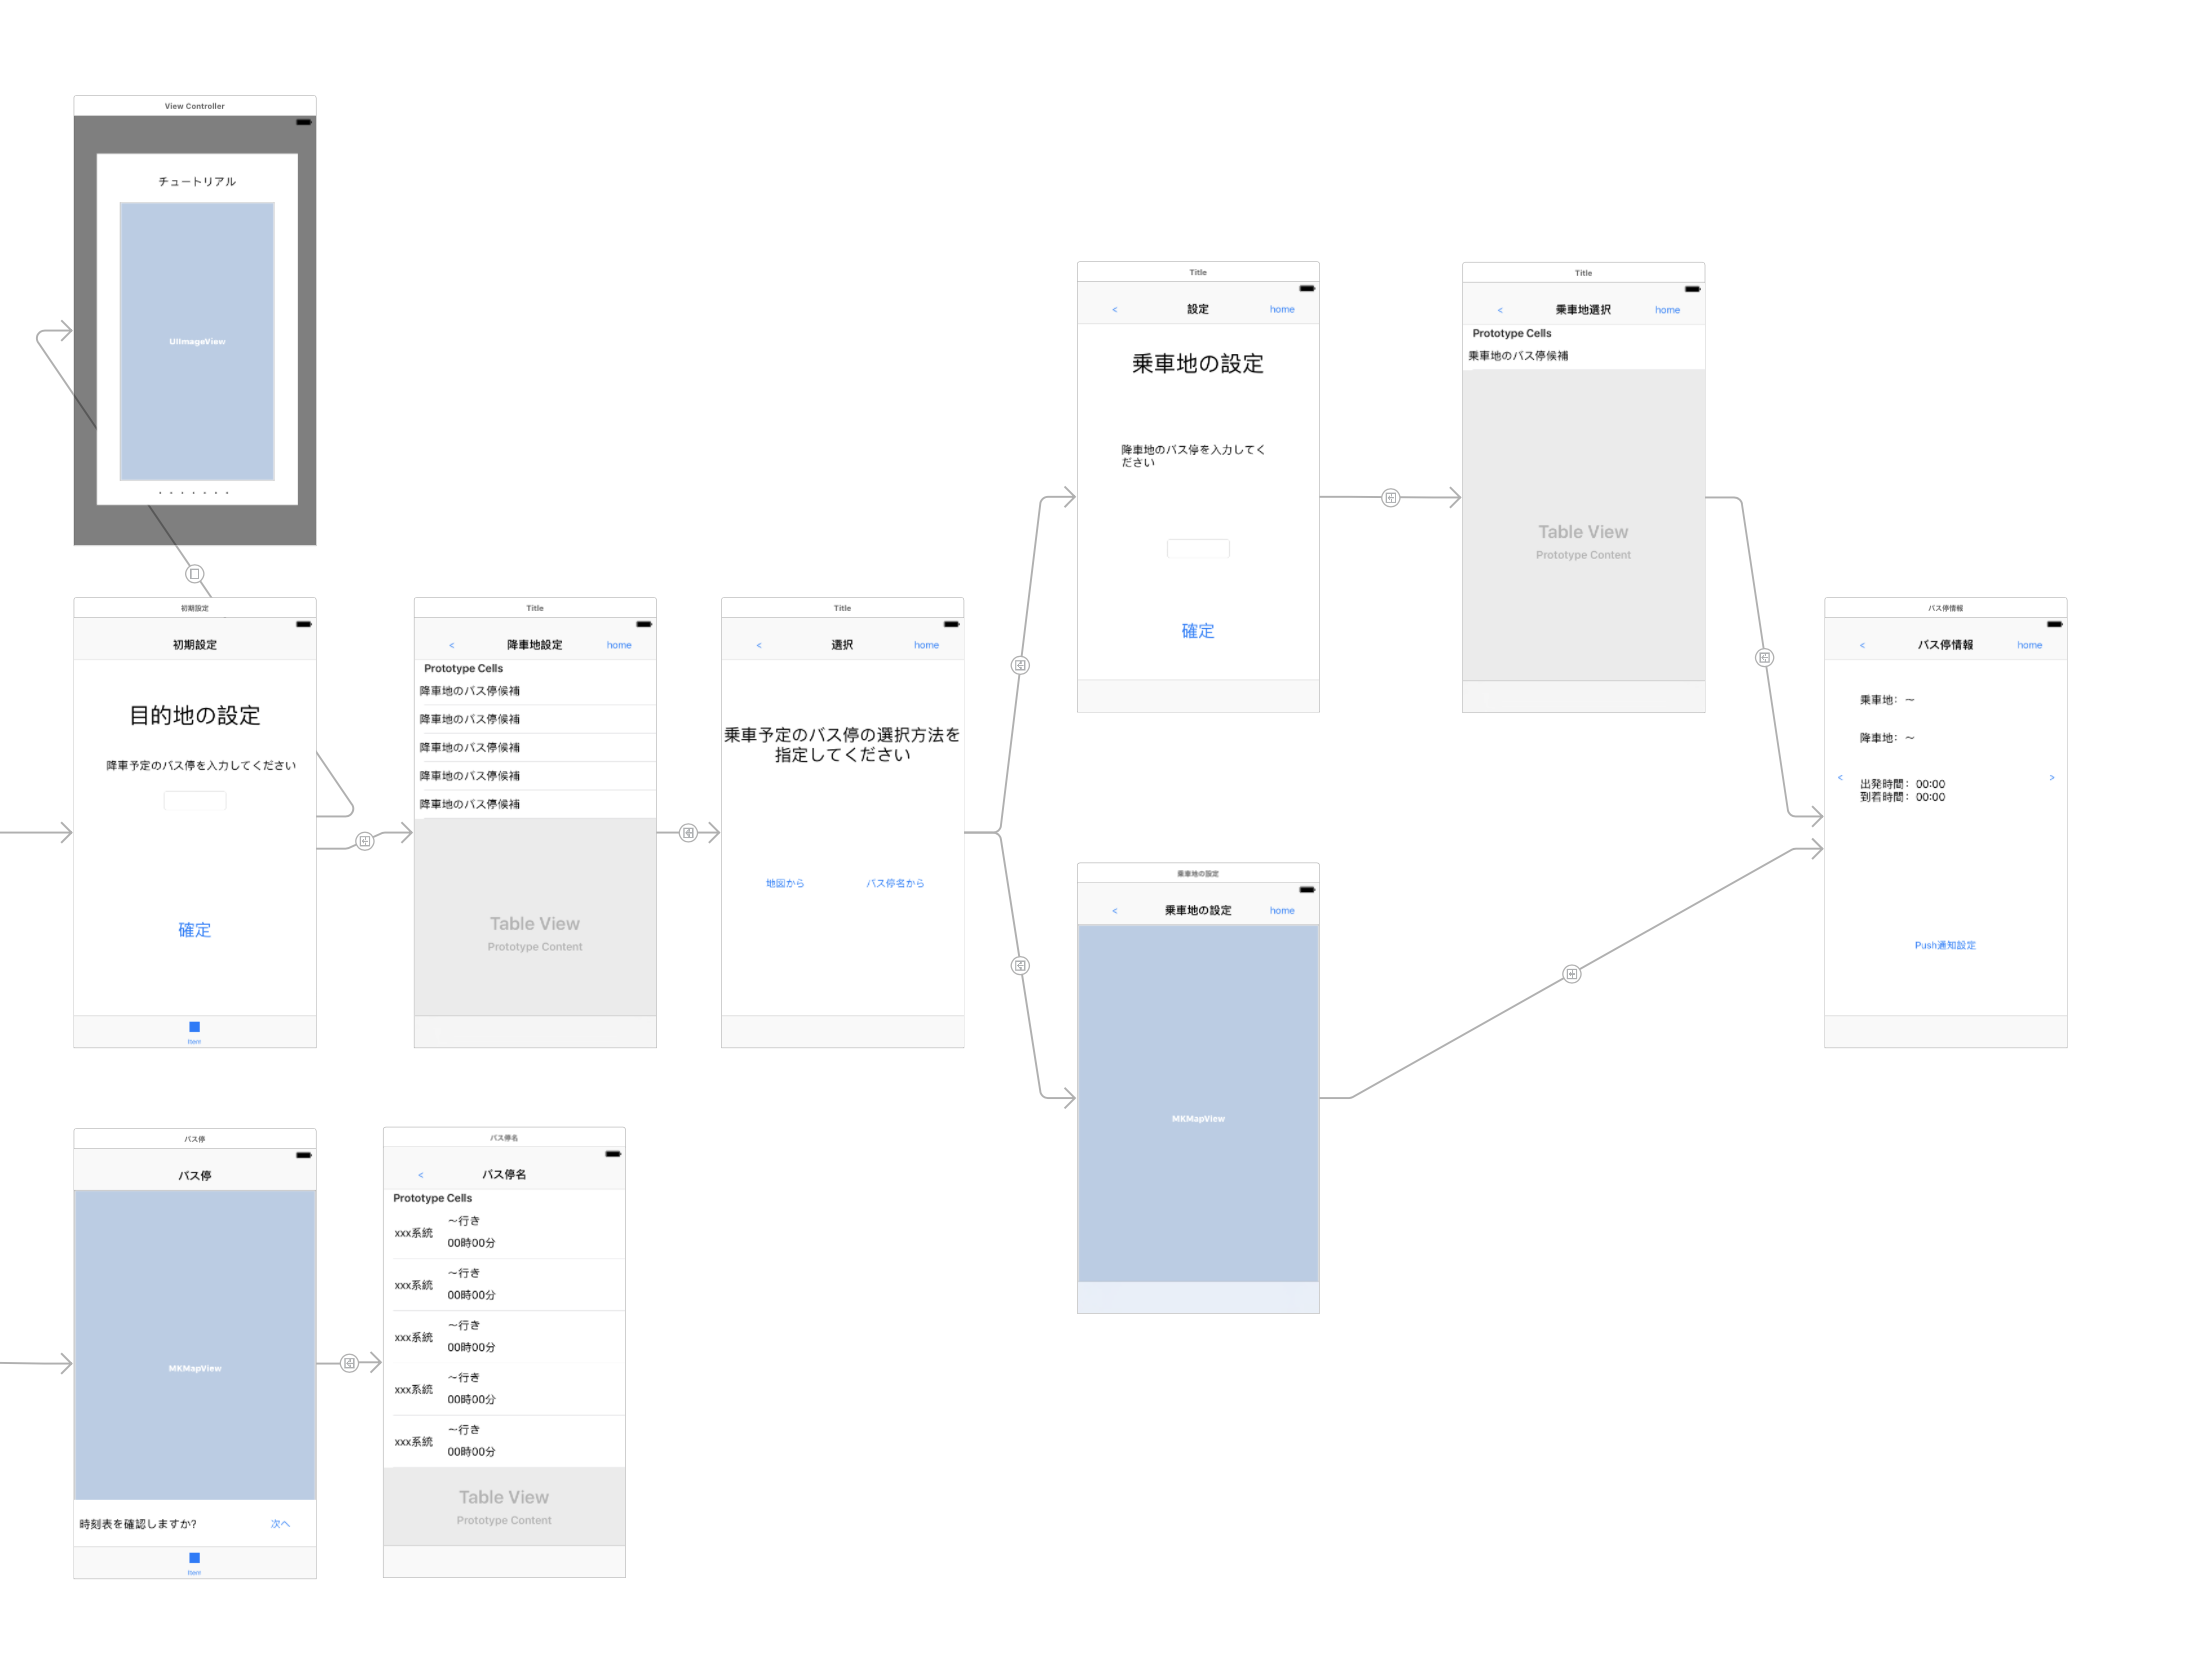
\includegraphics[clip,width=19cm,angle=90]{img/picture.png}
    \label{fig:senni}
  \end{center}
\end{figure}

\chapter{中間発表ポスター}
\begin{figure}[htbp]
  \begin{center}
    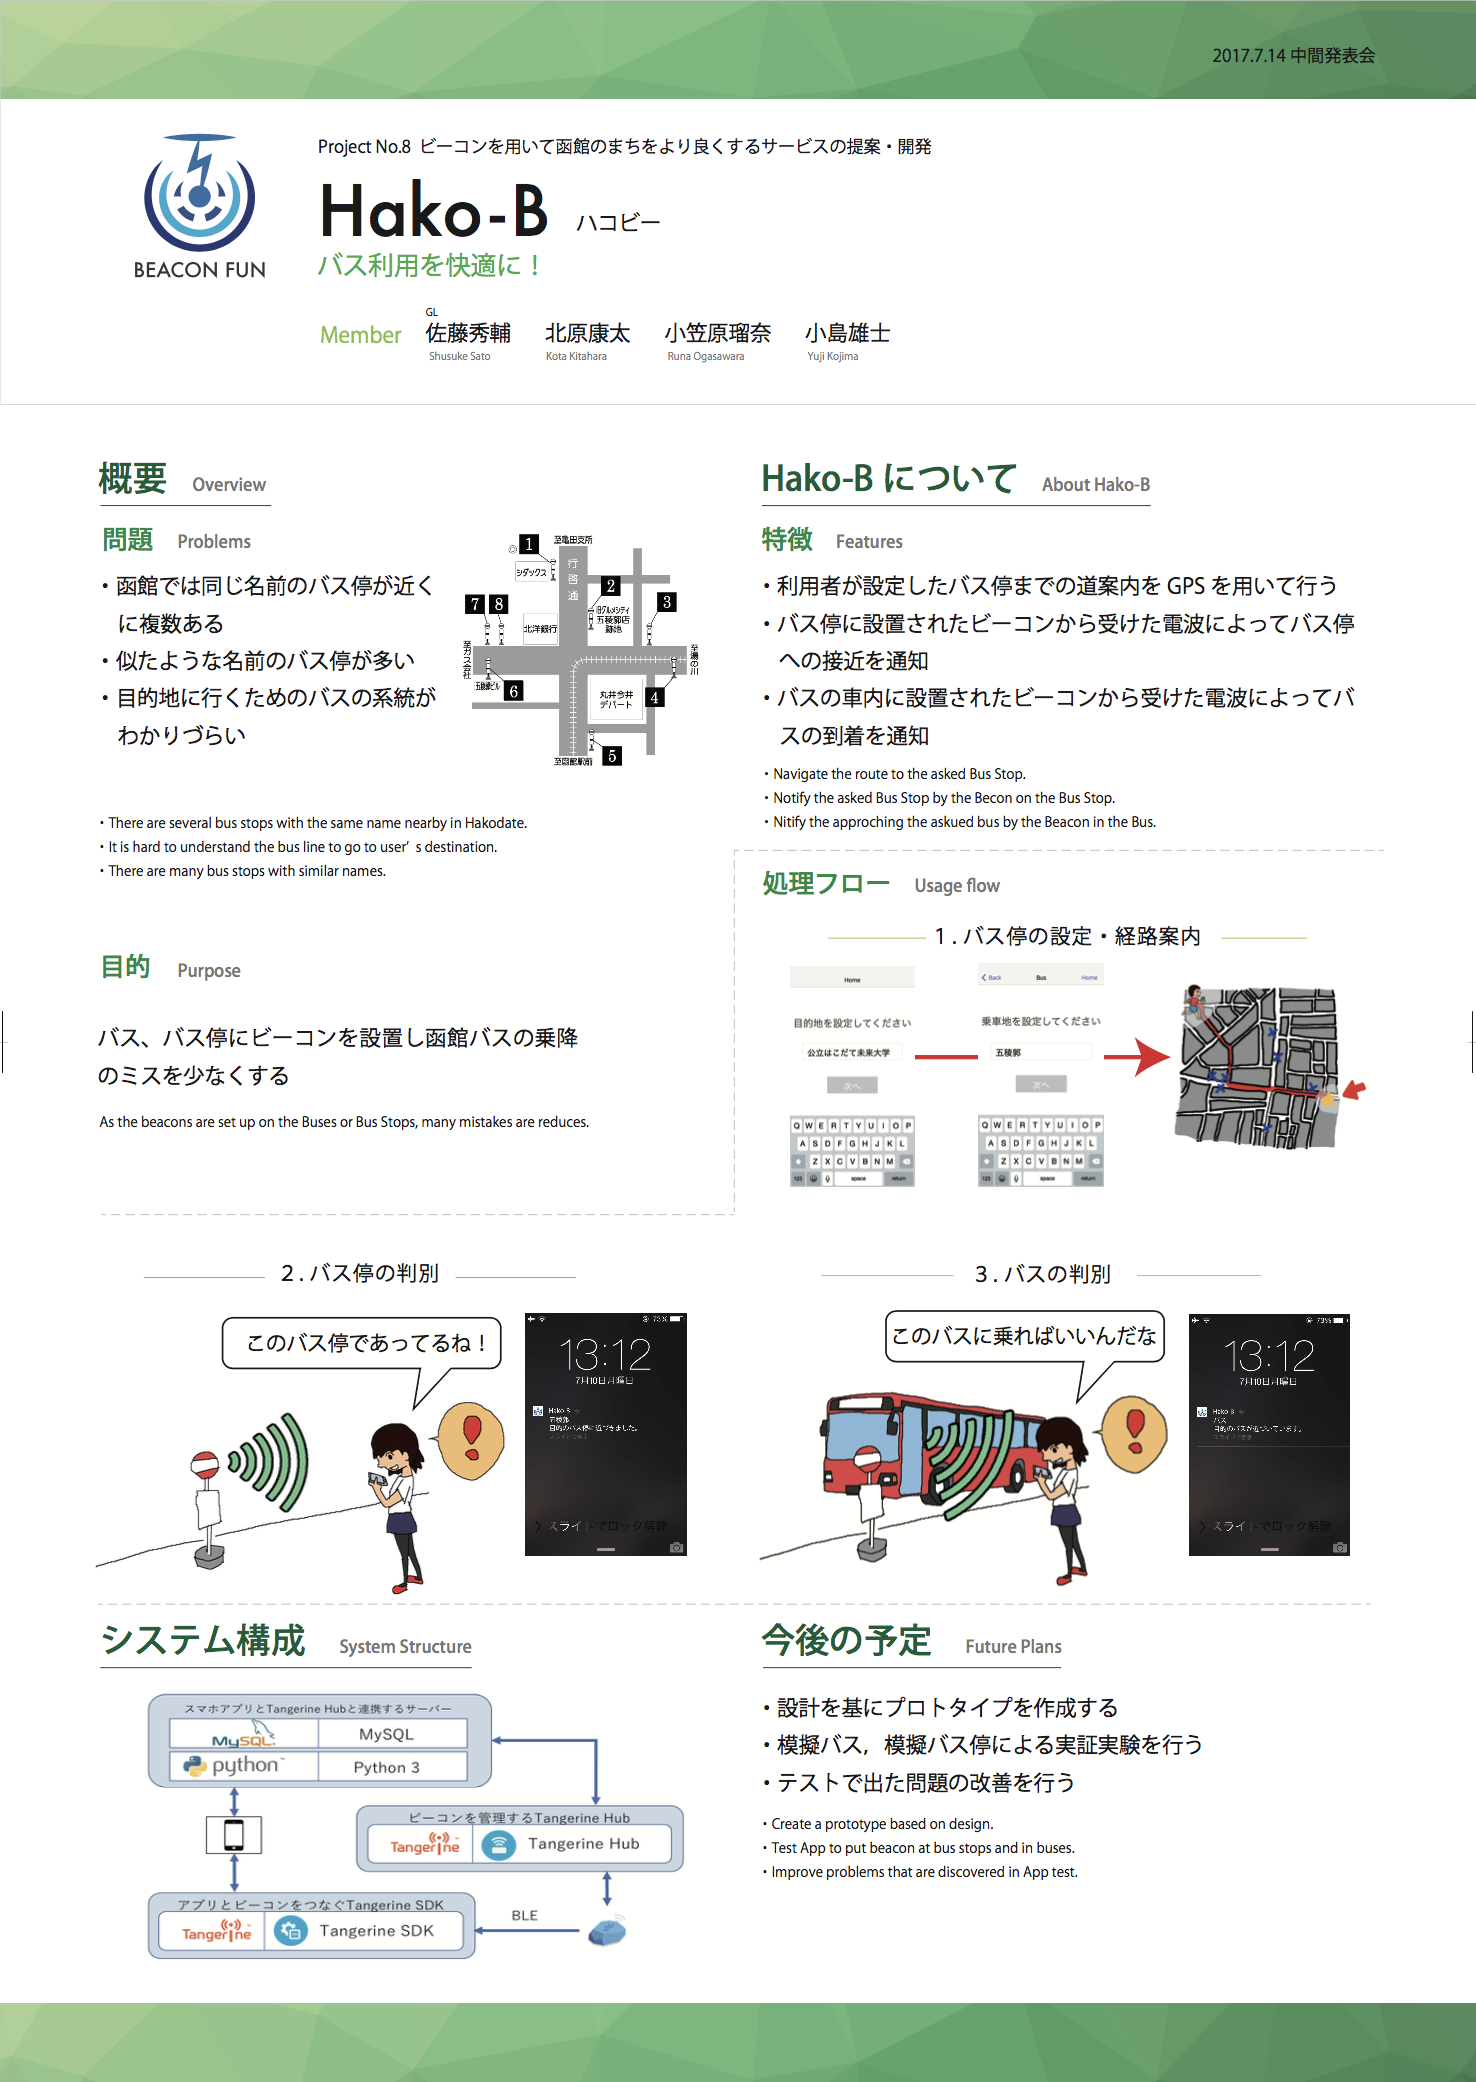
\includegraphics[clip,width=14cm]{img/poster.png}
    \label{fig:poster}
  \end{center}
\end{figure}

\chapter{最終発表ポスター}
\begin{figure}[htbp]
  \begin{center}
    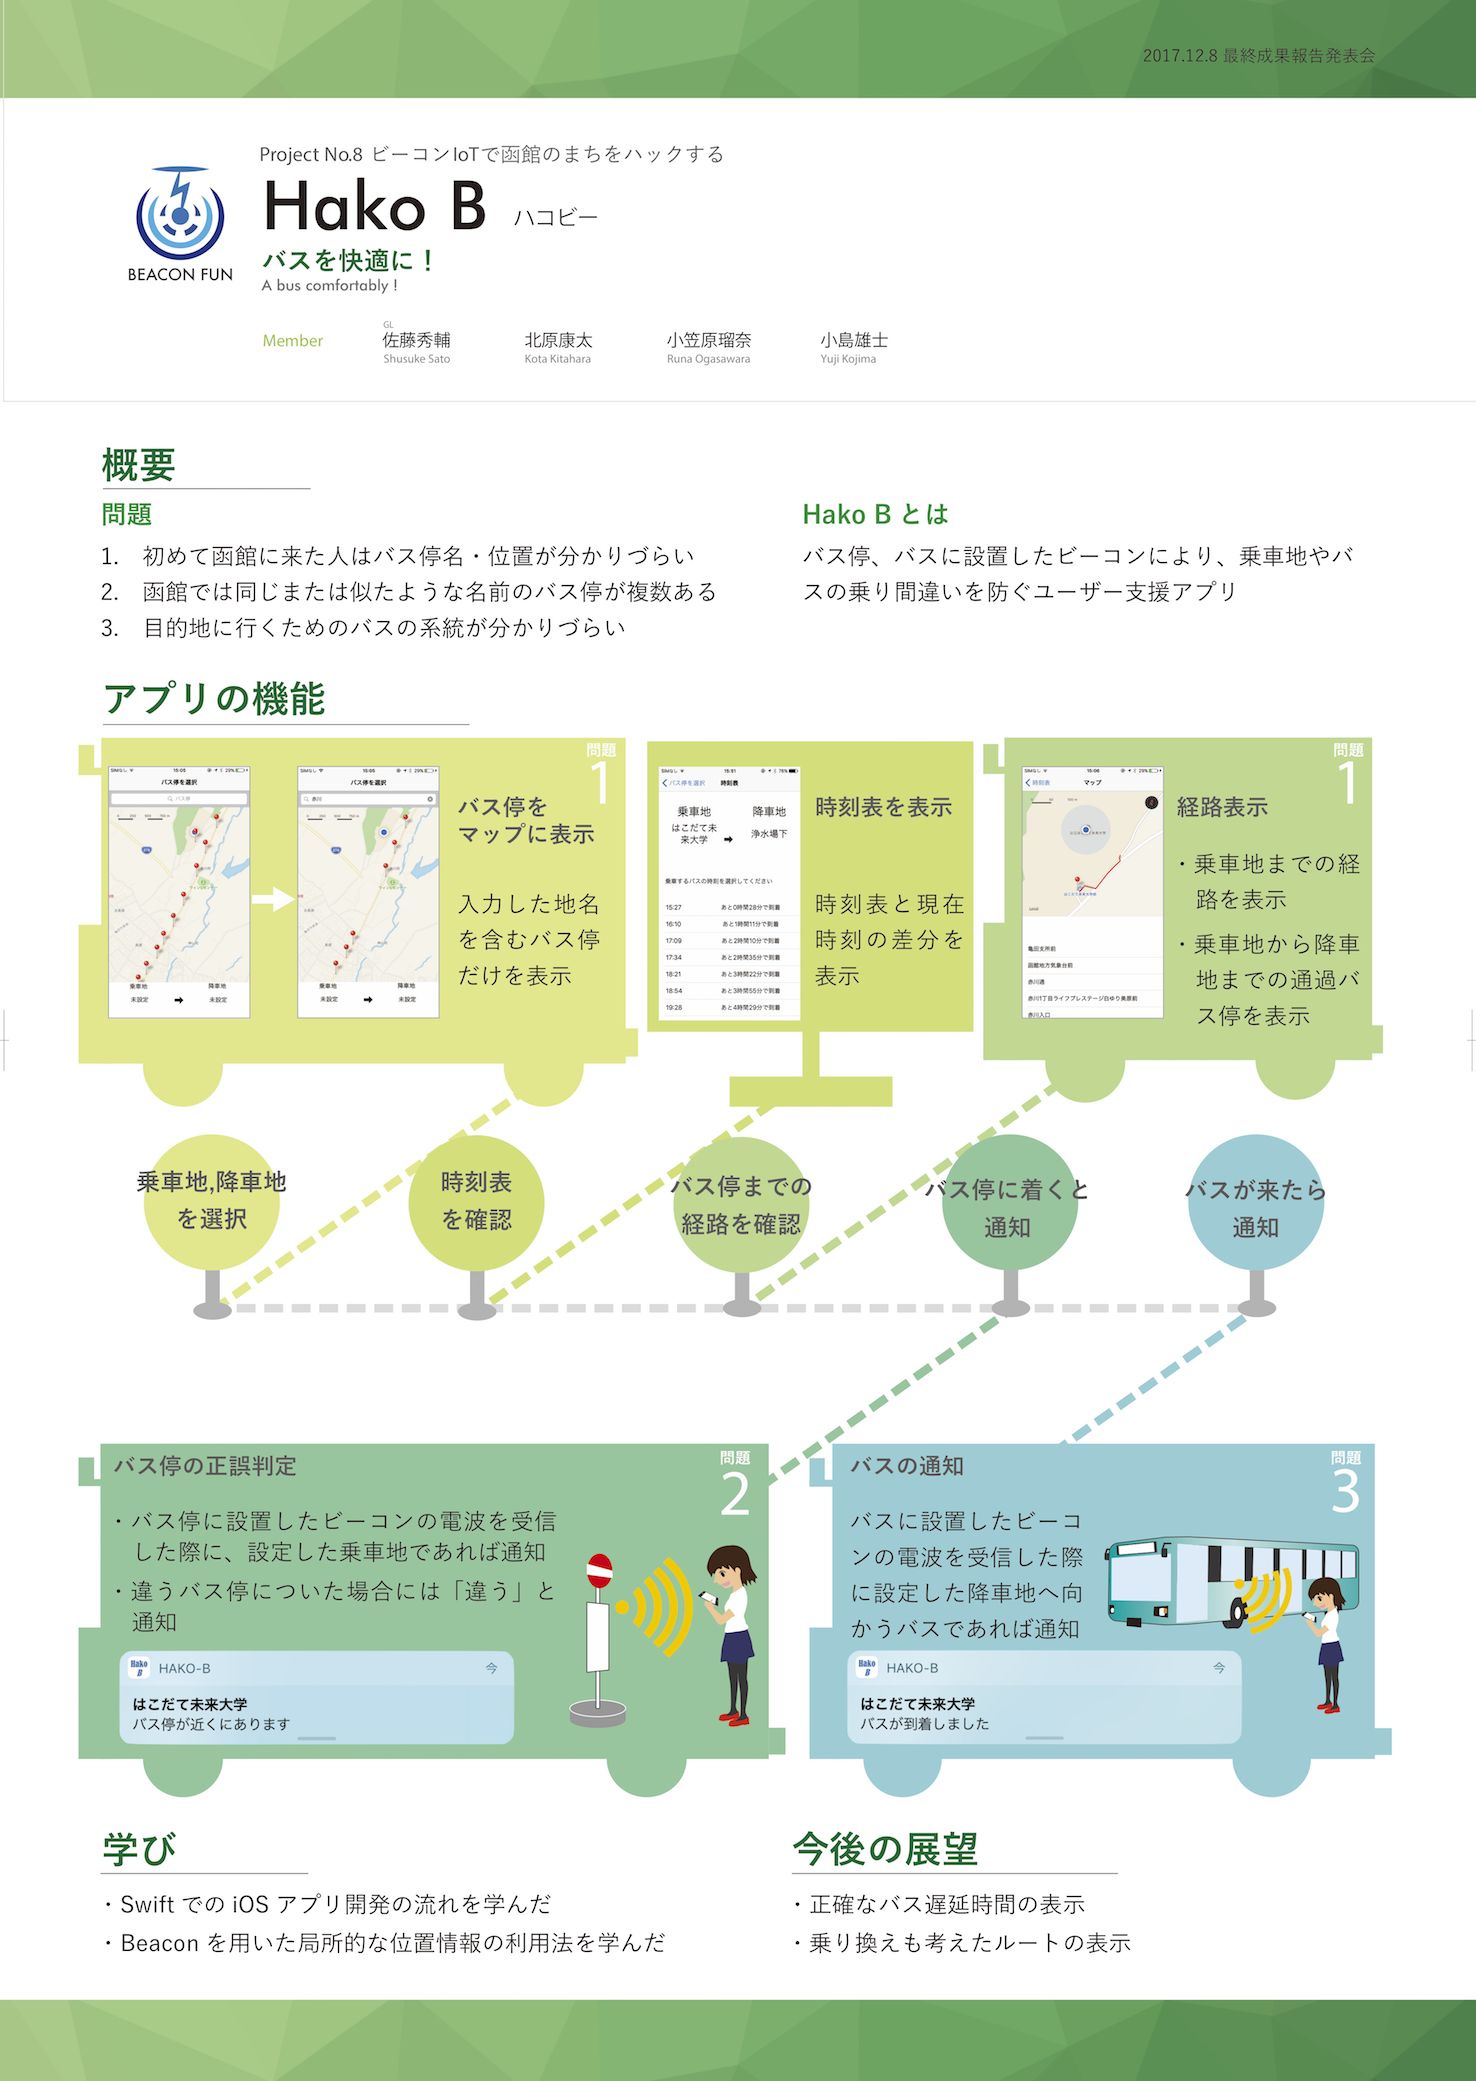
\includegraphics[clip,width=14cm]{img/final_poster.png}
    \label{fig:poster}
  \end{center}
\end{figure}
  
  %付録の終わり
  \end{appendix}
  
  
  %\backmatter
  
  \begin{thebibliography}{9}
    \bibitem{JohoWhitepaper} 総務省, 平成28年版 情報通信白書 第1部 特集 IoT・ビッグデータ・AI~ネットワークとデータが創造する新たな価値~
    http://www.soumu.go.jp/johotsusintokei/whitepaper/ja/h28/html/nc122530.html
  
    [last accessed 2017/7/24]
  \end{thebibliography}
  
  \end{document}
  